\documentclass[10pt]{article}
\usepackage{fontspec}
\usepackage{polyglossia}
\setdefaultlanguage{french}
\usepackage[a4paper,margin=2cm]{geometry}
\usepackage{url,hyperref}
\usepackage{siunitx}
\usepackage{schemabloc}
\usepackage{listings}
\usepackage{auto-pst-pdf}
\usepackage{pst-circ}
\usepackage{soul}
\usepackage{verbatim}
\usepackage{lmodern}
\usepackage{tikz}
\usepackage[european,cuteinductors,siunitx]{circuitikz}
\usepackage{xunicode,xltxtra}
\usepackage{graphicx}
\usepackage{amsmath}
\usepackage{minted}
\usepackage{multicol}
\title{
\includegraphics{../../../images/inp-enseeiht} \\ ~ \\ ~ \\ ~ \\ ~ \\
TP Composants}
\author{Guilhem Saurel}
\date{\today}
\renewcommand{\thesection}{\Roman{section}}
\renewcommand{\thesubsection}{\thesection .\alph{subsection}}
\begin{document}

 \begin{titlepage}
  \maketitle
  \tableofcontents
 \end{titlepage}

 \part{Transistors bipolaires}
  \section{Analyse des caractéristiques d’un transistor Bipolaire}
   \begin{center}
    Tracé de la caractéristique $I_c(V_{ce})$ : circuit et simulation
    
    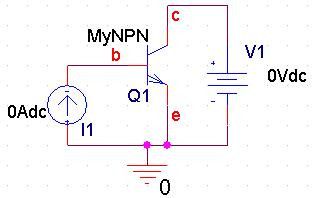
\includegraphics[width=8cm]{I-I_carac-stat-npn_ic-vce_circuit.jpg}
    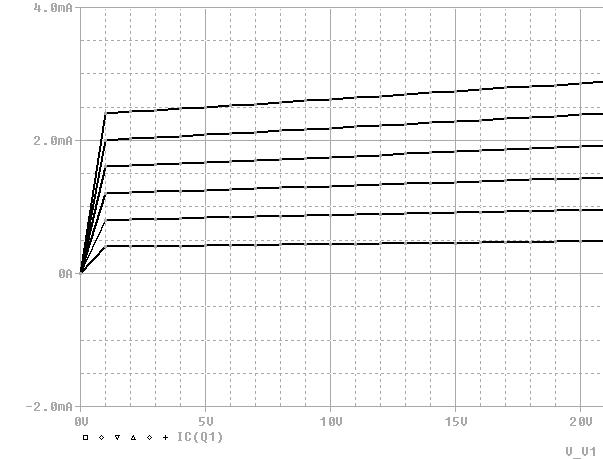
\includegraphics[width=8cm]{I-I_carac-stat-npn_ic-vce_simu.jpg}

    Tracé de la caractéristique $I_c(V_{be})$ : circuit et simulation

    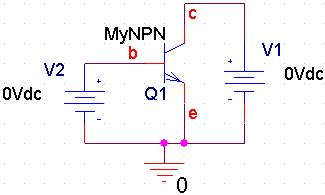
\includegraphics[width=8cm]{I-I_carac-stat-npn_ic-vbe_circuit.jpg}
    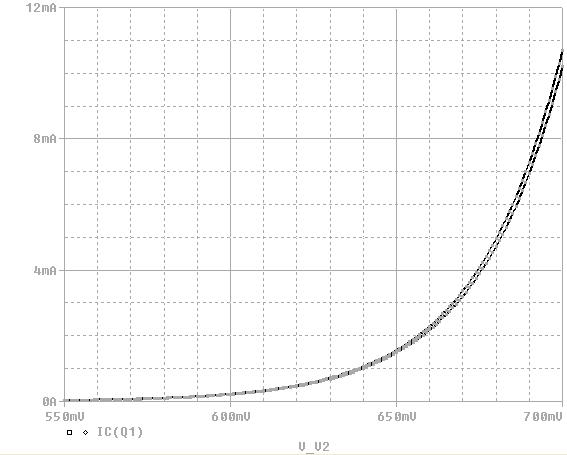
\includegraphics[width=8cm]{I-I_carac-stat-npn_ic-vbe_simu.jpg}
   \end{center}

  \section{Simulation d’un amplificateur Émetteur Commun}
   \subsection{Étude du point d’équilibre}
    Pour le calcul du point d’équilibre, on se place en continu, donc les
    condensateurs sont des coupe-circuit:
    \begin{center}
     \begin{circuitikz} 
      \draw
       (0,0) to[battery=$EC$] (0,6) -- (2,6)
        to[R=$R_{B1}$] (2,4) -- (2,2)
        to[R=$R_{B2}$] (2,0) -- (0,0)
       (4,3) node[npn] (npn) {}
       (2,3) -- (npn.base) node[anchor=south] {}
       (4,2) -- (npn.emitter) node[anchor=west] {}
       (4,4) -- (npn.collector) node[anchor=east] {}
       (2,6) -- (4,6) to[R=$R_C$] (4,4)
       (4,2) to[R=$R_E$] (4,0) -- (2,0)
      ;
     \end{circuitikz}
    \end{center}

    On commence par faire l’hypothèse que l’on peut négliger le courant de base,
    et que donc on peut obtenir la tension au niveau de la base avec la formule
    du pont diviseur sur les deux résistances de base: 
    $V_b = \cfrac{R_{b2}}{R_{b1} + R_{b2}} EC = 3.83$V

    La tension base-émetteur étant de $0.6$V, on a $V_e = V_b - 0.6 = 3.23$V.

    On en déduit le courant d’émetteur: $I_e = \cfrac{V_e}{R_e} = 1.47$mA.

    Et ensuite le courant de base: $I_b = \cfrac{I_e}{\beta + 1} = 3.66 \mu$A.

    Et enfin le courant de collecteur (même si on chipote un peu, là, parce qu’à
    un quart de pour-cent près, il est égal au courant d’émetteur…):
    $I_c = \beta I_b = 1.46$mA.

    Il ne manque plus que la tension du collecteur: $V_c = EC-R_c I_c = 8.05$V.

    On peut alors vérifier notre hypothèse: le courant de base ($3.66\mu$A)
    est bien négligeable devant le courant qui circule dans les résistances de
    base ($\cfrac{EC}{R_{b1}+R_{b2}} = 174\mu$A).

    Tout ceci est vérifié sous SPICE:

    \begin{center}
     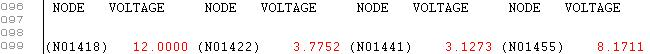
\includegraphics{I-II-a_pt-equi_out.jpg}

     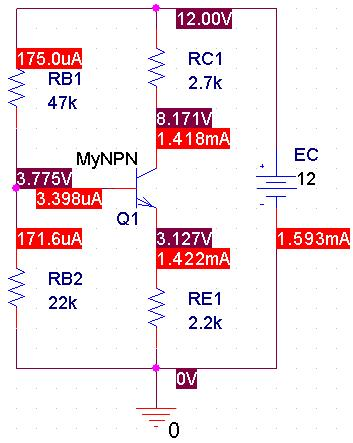
\includegraphics{I-II-a_pt-equi_circuit_et_valeurs.jpg}
    \end{center}

    On note un léger écart sur toutes les valeurs: c’est ce qui fait l’intérêt
    de la simulation, qui prend en compte des influences que l’on a l’habitude de
    négliger lors des calculs à la main.

   \newpage

   \subsection{Diagramme de Bode}
    \begin{center}
     Tracé du diagramme de Bode en amplitude du gain $G_V$ de 100Hz à 100MHz:

     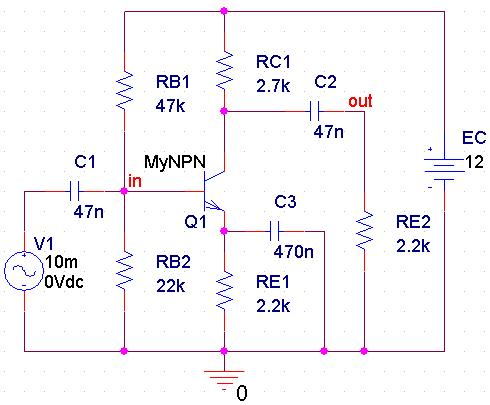
\includegraphics[width=8cm]{I-II-b_bode_circuit.jpg}
     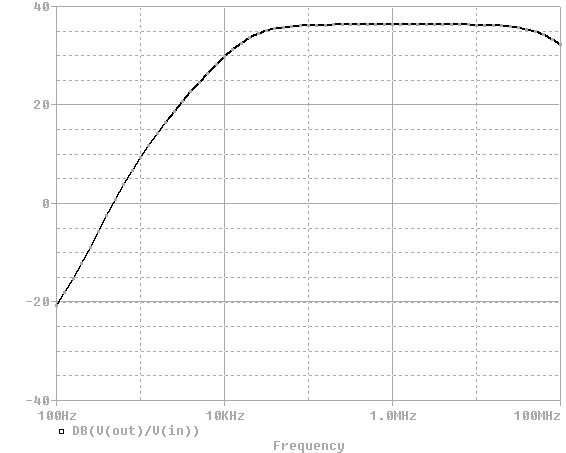
\includegraphics[width=8cm]{I-II-b_bode_simu.jpg}
     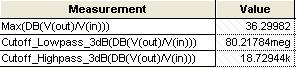
\includegraphics{I-II-b_bode_values.jpg}
    \end{center}
    La fréquence de coupure basse provient d’un filtre passe-haut entre la
    résistance série collecteur du transistor et le condensateur C2 ; sa valeur
    théorique est de $f_{CBF}= \cfrac{1}{2\pi 50\cdot 47\cdot 10^{-9}} = 67$kHz.

   \subsection{Influence de $C_e$ sur le gain}
    Pour ce montage à émetteur commun, le gain du circuit avec $C_e$ vaut $-g_m
    (RC1 \parallel RE2)$, mais si on l’enlève, il vaut $\cfrac{\beta_N(RC1
    \parallel RE2)}{r_\pi+\beta_N RE1}$.
    \begin{center}
     Tracé du même diagramme, sans $C_e$:

     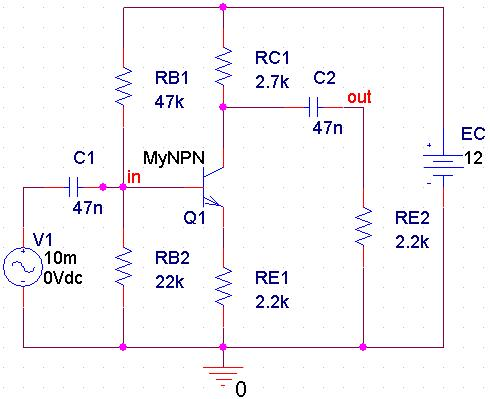
\includegraphics[width=8cm]{I-II-c_sans-ce_circuit.jpg}
     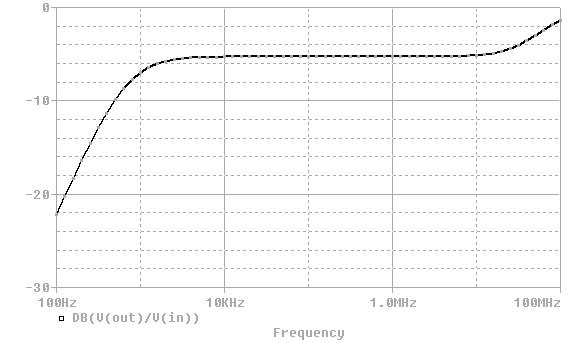
\includegraphics[width=8cm]{I-II-c_sans-ce_simu.jpg}
    \end{center}
    Il apparait assez clairement que le gain de plateau (anciennement à 36dB) a
    chuté de 40dB.
   
   \newpage
   \subsection{Limite de linéarité}
    Avec une analyse temporelle et en augmentant progressivement l’amplitude de
    la tension d’entrée, il apparait une valeur limite aux alentours de 40mV:
    \begin{center}
     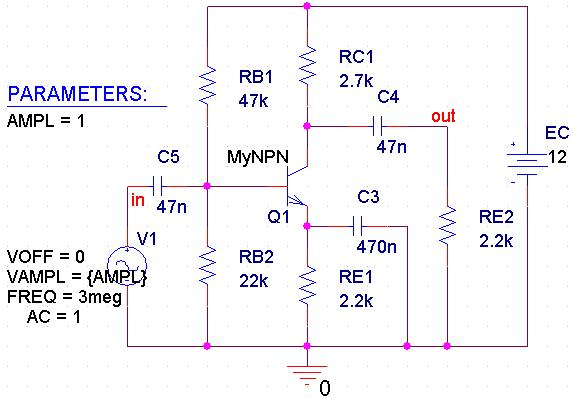
\includegraphics[width=8cm]{I-II-d_vin-max_circuit.jpg}
     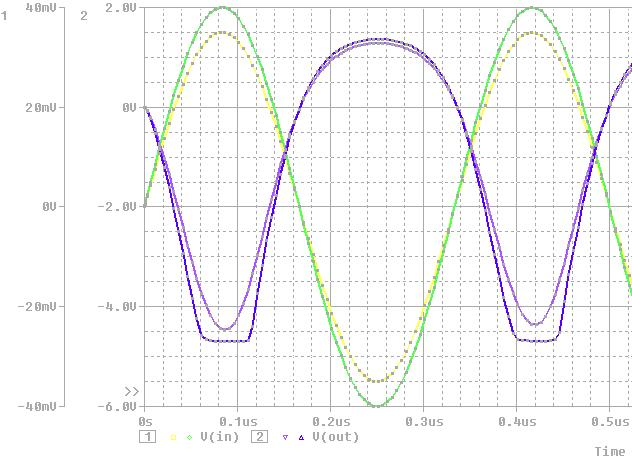
\includegraphics[width=8cm]{I-II-d_vin-max_simu.jpg}
    \end{center}

 \newpage
 \part{Transistor MOS}
  \section{Définition du modèle des transistors MOS}
   Fichier «mos.lib» final:
   \inputminted[linenos]{bash}{mos.lib}

  \section{Dimensionnement des transistors}
   \subsection{Largeur du transistor M2}
    \begin{center}
     Tracé de $I_{DS}(W)$:

     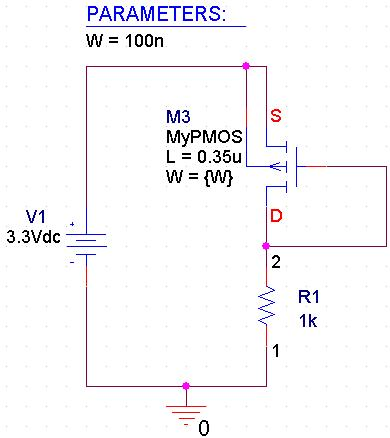
\includegraphics[width=8cm]{II-II-a_is-w_circuit.jpg}
     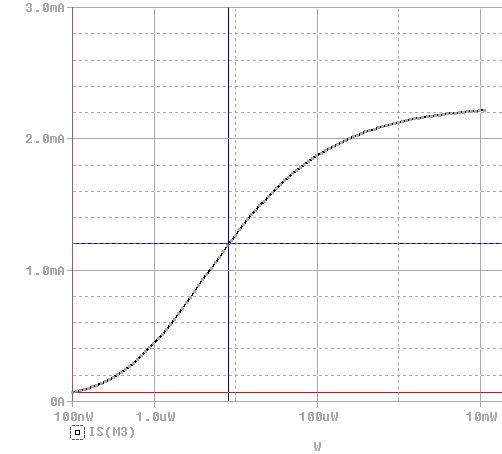
\includegraphics[width=8cm]{II-II-a_is-w_simu.jpg}
     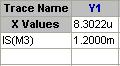
\includegraphics{II-II-a_is-w_values.jpg}
    \end{center}
    La largeur du transistor recherchée est donc $W_{M2}=8.30\mu$m.

   \subsection{}

   \subsection{Largeur du transistor M3}
    Le courant $I_{DS}$ étant directement proportionnel à la largeur $W$ dans la
    zone considérée, pour que M3 génère un courant deux fois moins important que
    M2, il suffit de diviser sa largeur par deux: $W_{M3}=4.15\mu$m.

   \subsection{Tension de seuil}
    $V_{T0} = \Phi_T + \gamma \sqrt{\Phi_T} \pm \lvert \Phi_{MS} \rvert$.

    Pour un MOS N, on a donc théoriquement $V_{T0} = 0.837+0.18 = 0.917$V, et
    SPICE nous donne 1.044V ; et pour un MOS P, $V_{T0} = 0.837-0.9 = -0.063$V
    et SPICE nous donne -0.0707V.

   \subsection{Charges à implémenter}
    Pour le MOS N, il faut abaisser la tension grâce à un dopage de type P de
    densité $N_A \delta = \cfrac{\varepsilon_{ox} \Delta V}{t_{ox} q}$.

    Et pour le MOS P, il nous faudra $N_D \delta = \cfrac{\varepsilon_{ox}
    \Delta V}{t_{ox} q}$.

    Dans les deux cas, il faut modifier empiriquement la valeur théorique en
    effectuant des simulations. Au final, les deux sont de l’ordre de $1.2\cdot
    10^{12}$.

  \section{Fonctionnement de l’amplificateur}
   \subsection{Point de fonctionnement du circuit}
    \begin{center}
     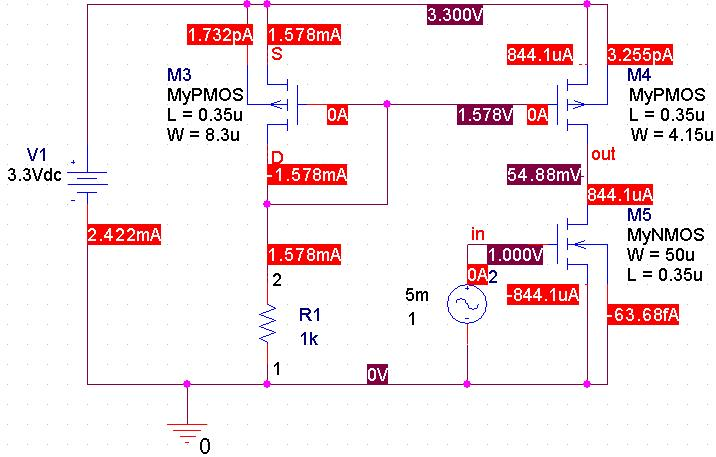
\includegraphics[width=16cm]{II-III-a_bias-point_circuit-et-valeurs.jpg}
    \end{center}

   \subsection{Gain en tension}


 \newpage
 \part{Annexes}
  \appendix
  \section{Fichier Scilab}
   Voici le fichier Scilab dans lequel tous les calculs sont faits :
   \inputminted[linenos]{matlab}{calculs.sci}

\end{document}
